\documentclass{beamer}

\usepackage{graphicx}
\usepackage{beamerthemesplit}
%\usepackage{footnote}
\usepackage[normalem]{ulem}
\title{A path to OpenAFS 2.0: rxgk, IPv6, and more}
\author{Benjamin Kaduk \\ \url{kaduk@mit.edu} \url{bkaduk@akamai.com}}
\date{20 August, 2015}

\begin{document}

\AtBeginSection[]
{
    \begin{frame}
	\tableofcontents[currentsection]
    \end{frame}
}

\frame{\titlepage}

\section{Roadmap}

\begin{frame}[fragile]
\frametitle{Things we want}
\begin{itemize}
\item{rxgk\hphantom{?}}
\item{IPv6 support}
\item{read-write replication}
\item{per-file ACLs}
%\vphantom{\item{\ldots}}
\end{itemize}
\end{frame}

\begin{frame}
\frametitle{Things we get}
\begin{itemize}
\item{rxgk?}
\pause
\item{\sout{IPv6 support}}
\pause
\item{\sout{read-write replication}}
\pause
\item{\sout{per-file ACLs}}
\pause
\item{\ldots}
\end{itemize}
\end{frame}

\subsection{History}

\begin{frame}
That's where we want to be (and where we think we'll actually be able to
get to).

\vspace{1em}
In order to get there, we have to know where to start --- where are we
coming from?
\end{frame}

\begin{frame}[fragile]
\frametitle{History}
People have wanted rxgk for longer than I've been using AFS!

\vspace{1em}
Back in 2006, the Elders published
\url{https://www.openafs.org/pages/no-more-des.html}.
\begin{quote}
After the 1.6 release, the build system will be modified to build OpenAFS
without kaserver unless it is specifically requested.

The OpenAFS Elders endorse the development of the rxk5 and rxgk security
classes in order to enable the use of Kerberos 5 ciphers other than single DES
for both authentication and data security between AFS clients and servers.

When OpenAFS is capable of supporting Kerberos 5 with non-DES ciphers the
major version number will be changed to "2".
\end{quote}
\end{frame}

\begin{frame}
\frametitle{IPv6}
\begin{itemize}
\item{OpenAFS is getting left behind}
\item{World is running out of v4 addresses}
\item{IPv6 is more and more common
	\begin{itemize}
	\item{cell networks}
	\item{home networks, too!}
	\item{Some ISPs charging more for v4 service}
	\end{itemize}
}
\item{v6 support is more than just replacing 32 bits with 128 bits}
\pause
\item{and more than just keeping both and a way to choose}
\item{(but we do still need to bump the vldb format to do anything)}
\end{itemize}
\end{frame}

\begin{frame}
\frametitle{IPv6}
I'm not an expert on IPv6 for AFS; talk to Jeff or Mike or Simon
or some number of other people who know more.

But\ldots
\begin{itemize}
\item{privacy addresses --- callbacks might not be deliverable!}
\item{larger minimum packet sizes; rx must adapt its ideas of MTU handling}
\item{Much larger physical packets possible, but rx jumbograms suck}
\item{fragmentation is not automatic --- must be prepared to resend
	in smaller chunks}
\item{Will the OS let you get the ICMPv6 fragmentation needed notices?}
\item{everybody becomes multihomed}
\end{itemize}
\end{frame}
\begin{frame}
\frametitle{IPv6}
\begin{itemize}
\item{Many, many RPCs to update}
\item{We're already ``in the middle of'' and RPC refresh \ldots for the
	past five\footnote{maybe more?} years}
\item{rxdebug}
\item{happy eyeballs}
\end{itemize}
\end{frame}

\section{What's in 1.8?}

\begin{frame}[fragile]
\frametitle{Why 1.8?}
\begin{itemize}
\item{\verb+openafs-stable-1_6_x+ was branched on August 10, 2010}
\item{4658 commits on master since then, but only 2033 commits on
1.6 since then.  (Most of the commits on 1.6 are cherry-picks from
master, but not all; I didn't write the script to check.)}
\item{Those other 2.5k commits have some useful features in them!}
\item{\verb+master+ is actually pretty usable right now; rxgk and
whatnot will probably break things temporarily.  A new release gives
a stable baseline to start from.}
\item{We're also overdue for some breaking/intrusive changes that
should only be done at a major release boundary.}
\end{itemize}
\end{frame}

\begin{frame}
\frametitle{What's in 1.8?}
Already on master:
\begin{itemize}
\item{Code cleanup/robustness (e.g., from static analyzers, compiler
warnings fixes, and general refactoring) --- thanks, Simon!}
\item{libtool in the build system for more reliable shared libraries,
and other build system cleanup}
\item{pthreaded dbservers}
\item{Greatly reduced krb5 dependencies}
\item{More reliable autoconf logic}
\item{Windows stuff is quite different}
\item{Some parts of the documentation are not embarassing}
\item{\sout{Improvements} changes to the rx stack (again, thanks, Simon!)}
\item{libroken and libhcrypto from Heimdal}
\item{Cache bypass on Linux}
\item{OpenAFS Portable Runtime (opr) --- thanks, Simon!}
\item{Some afsd.fuse improvements}
\end{itemize}
\end{frame}
\begin{frame}
\frametitle{What's in 1.8?}
Already on master:
\begin{itemize}
\item{cmd refactoring}
\item{Something resembling a test suite framework}
\item{New default for ihandle sync-ing behavior}
\item{Some bosserver refactoring}
\item{Ability to control ugen/ubik client flags more closely}
\item{memcache improvements}
\item{rxgen per-opcode stats}
\item{openafs-client.conf and openafs-server.conf}
\item{opr\_Assert() vs. opr\_Verify()}
\item{More dbserver threads by default}
\item{buserver uses libutil's logging (format changes)}
\item{other changes to server logging, rotation}
\item{CacheTruncateDaemon improvements}
\item{Use Heimdal's rand-fortuna in the kernel}
\end{itemize}
\end{frame}
\begin{frame}
\frametitle{What's in 1.8?}
Already on master:
\begin{itemize}
\item{ptserver wire format arrays' length is capped}
\item{bos, pts emit error messages on stderr (not stdout)}
\item{vos remaddrs}
\item{opr\_softsig}
\end{itemize}
\end{frame}

\begin{frame}
\frametitle{In gerrit ready to be merged}
% 38 changes
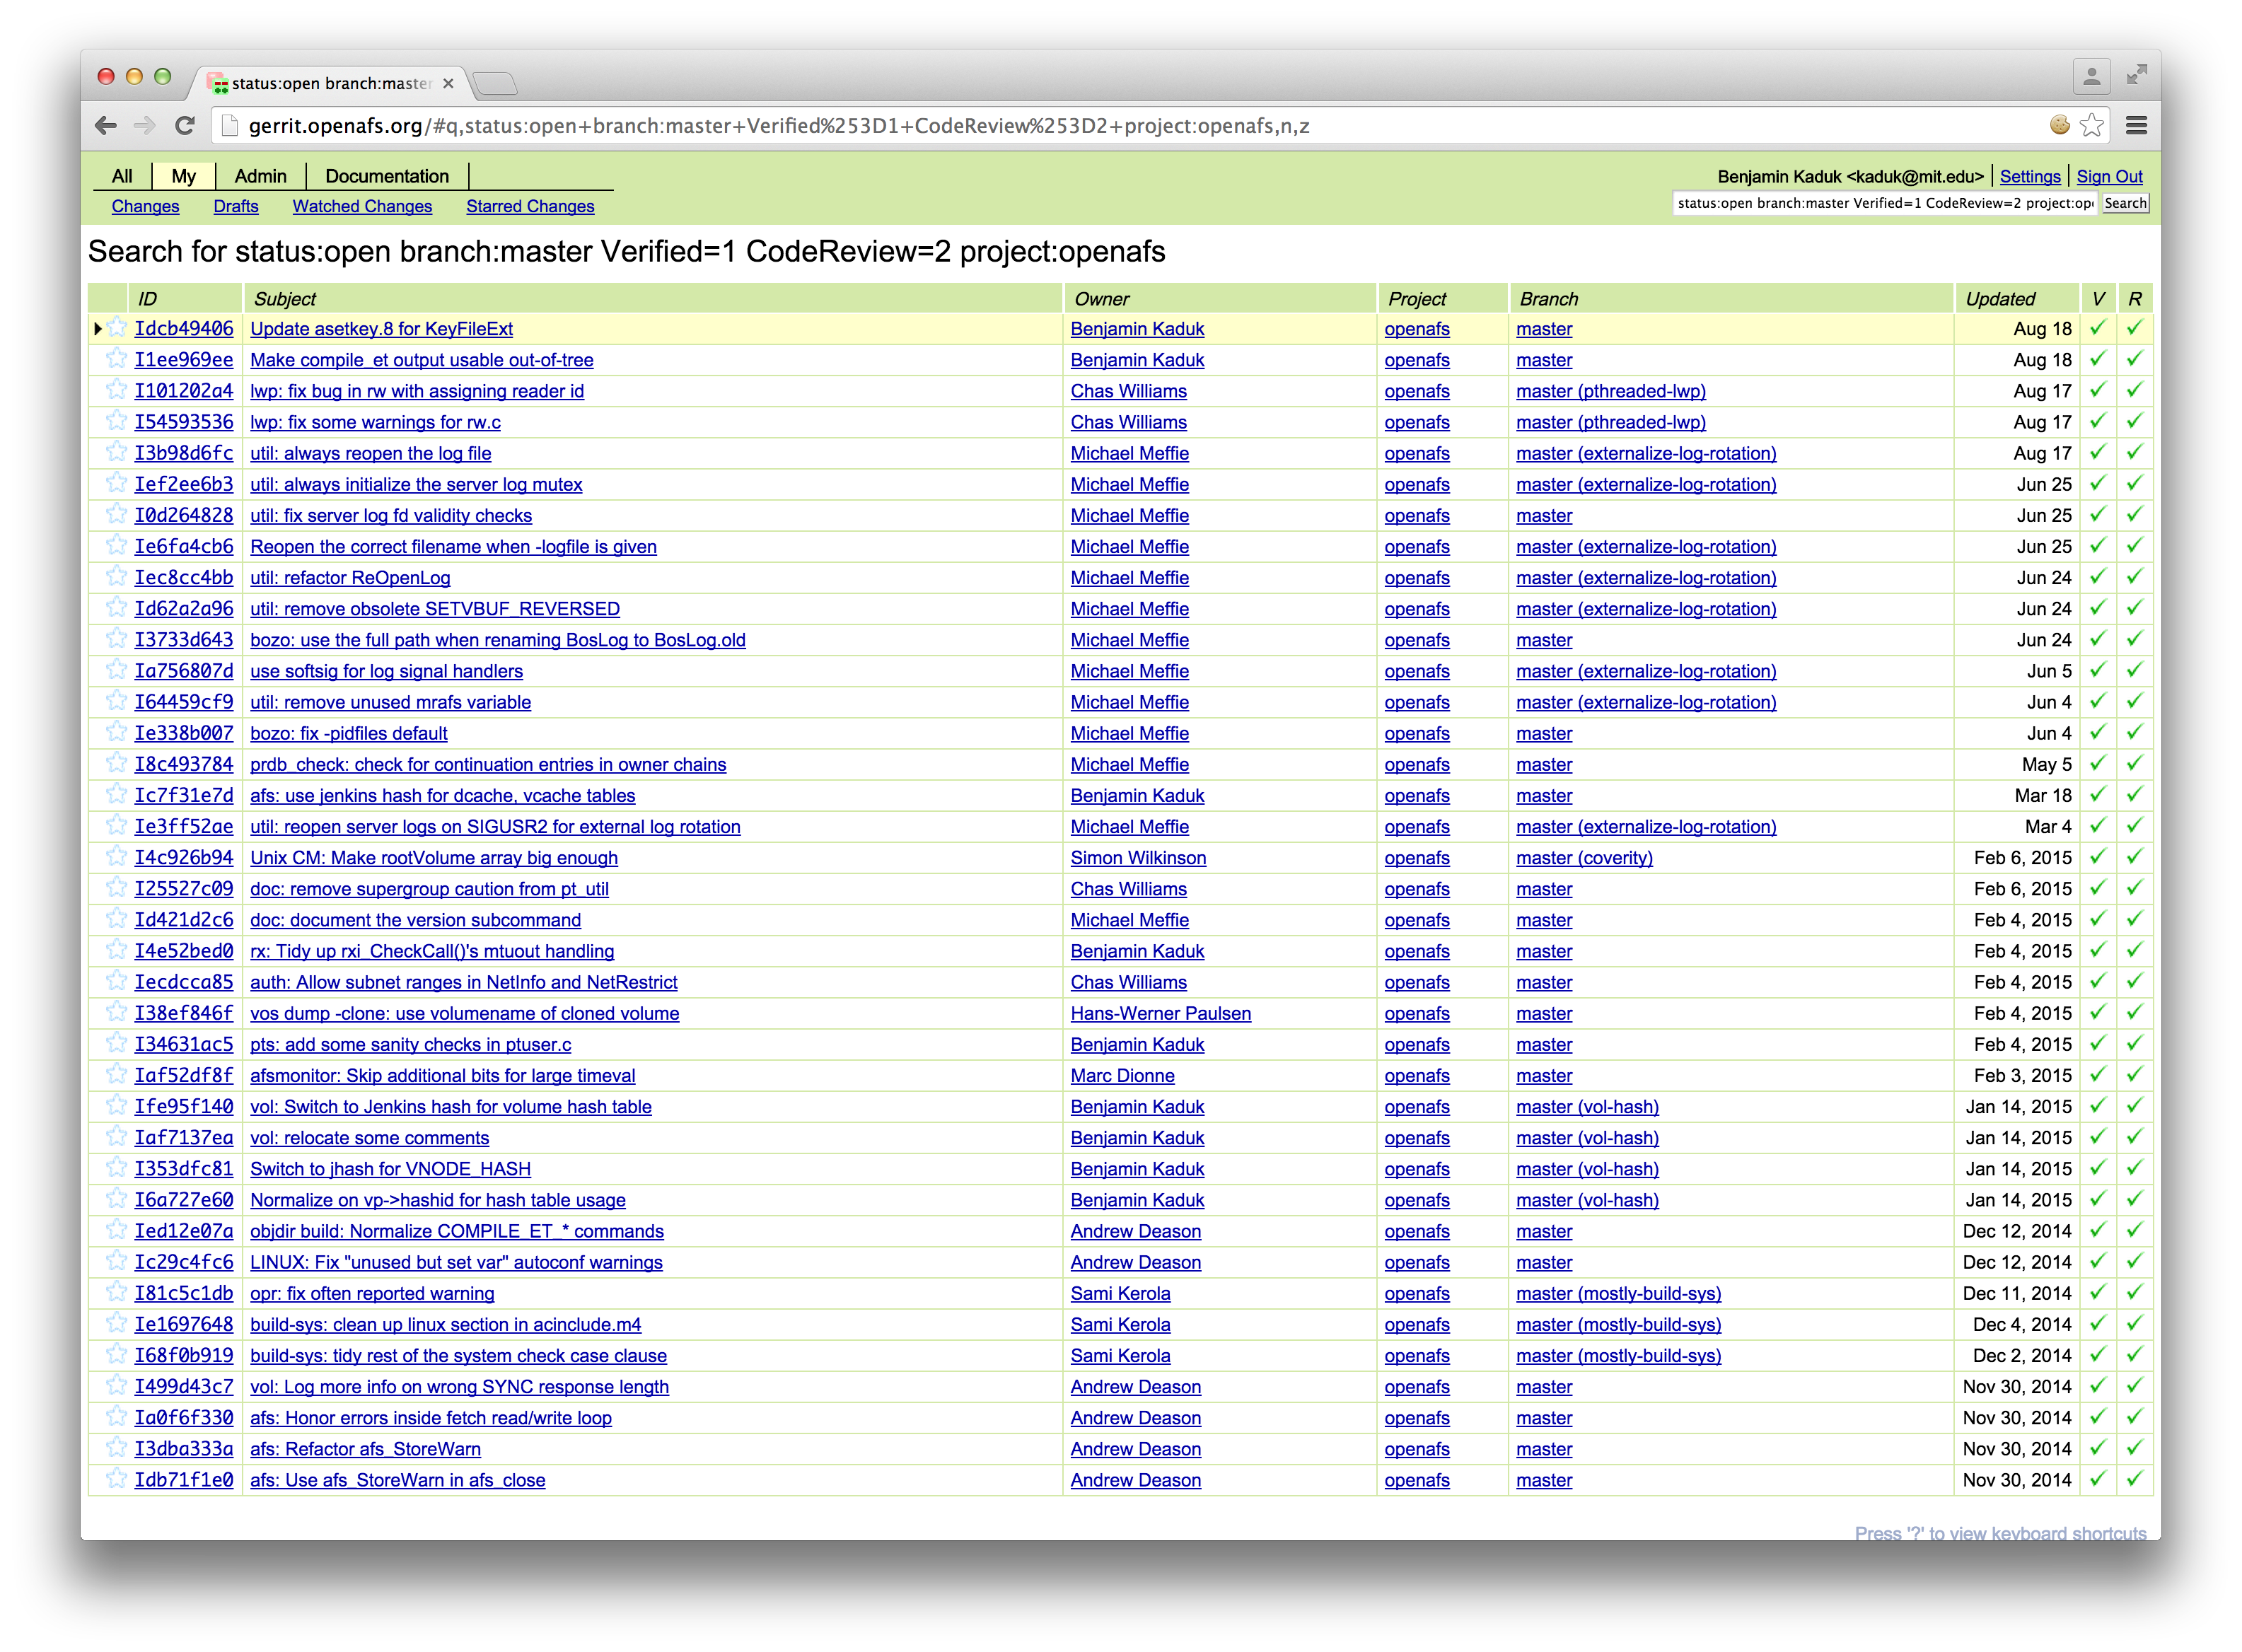
\includegraphics[width=4in]{gerrit-approved}
\end{frame}

\begin{frame}
\frametitle{In gerrit ready to be merged}
38 changes with good code review.
\vspace{1em}
Need to actually get merged.
\end{frame}

\begin{frame}
\frametitle{In gerrit ready to be merged}
\begin{itemize}
\item{Jenkins hash in volume, vnode, vcache, dcache hash tables}
\item{Subnet ranges in NetInfo/NetRestrict}
\end{itemize}
\end{frame}

\begin{frame}
\frametitle{In gerrit needing review}
%54 changes
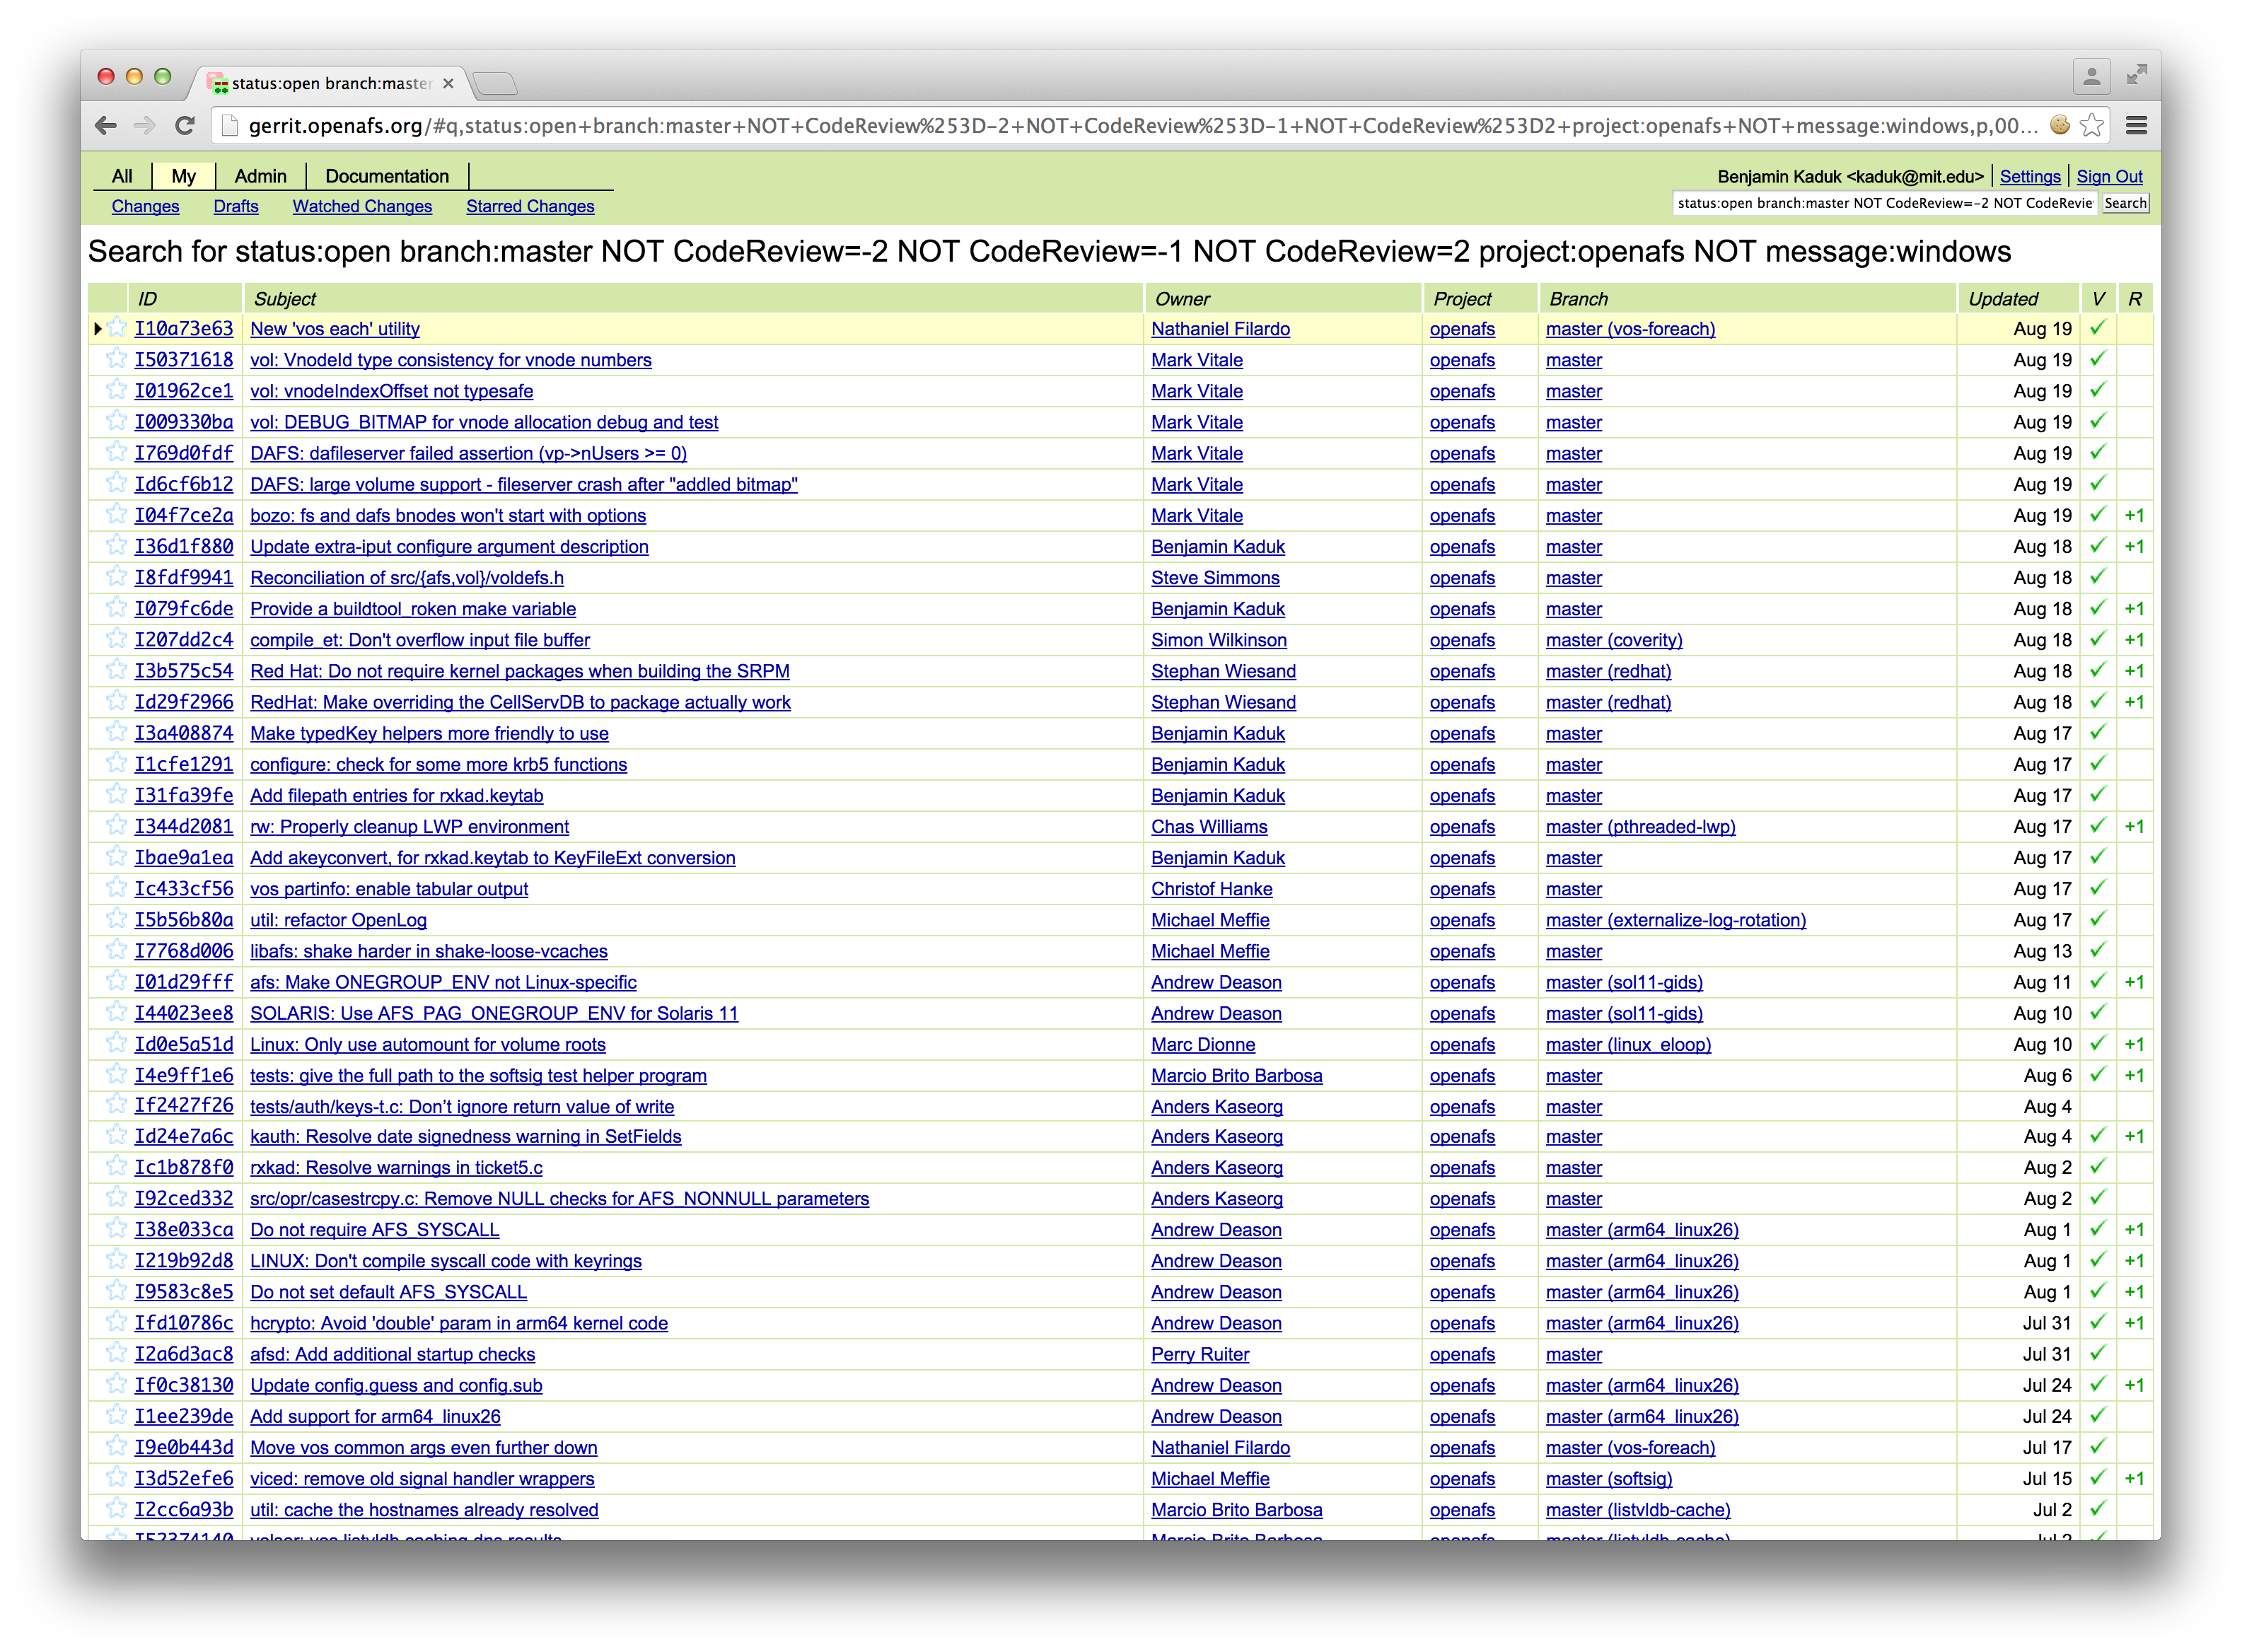
\includegraphics[width=4in]{gerrit-needsreview}
\end{frame}

\begin{frame}
\frametitle{In gerrit needing review}
54 changes (just barely on two pages)
\begin{itemize}
\item{update bos restricted mode}
\item{encrypt inter-volser traffic}
\item{Revert "Lockless path through afs\_linux\_dentry\_revalidate"}
\item{afs: Don't retry timed-out RW operations forever}
\end{itemize}
\end{frame}

\begin{frame}
\frametitle{In gerrit needing rework}
% 33 changes
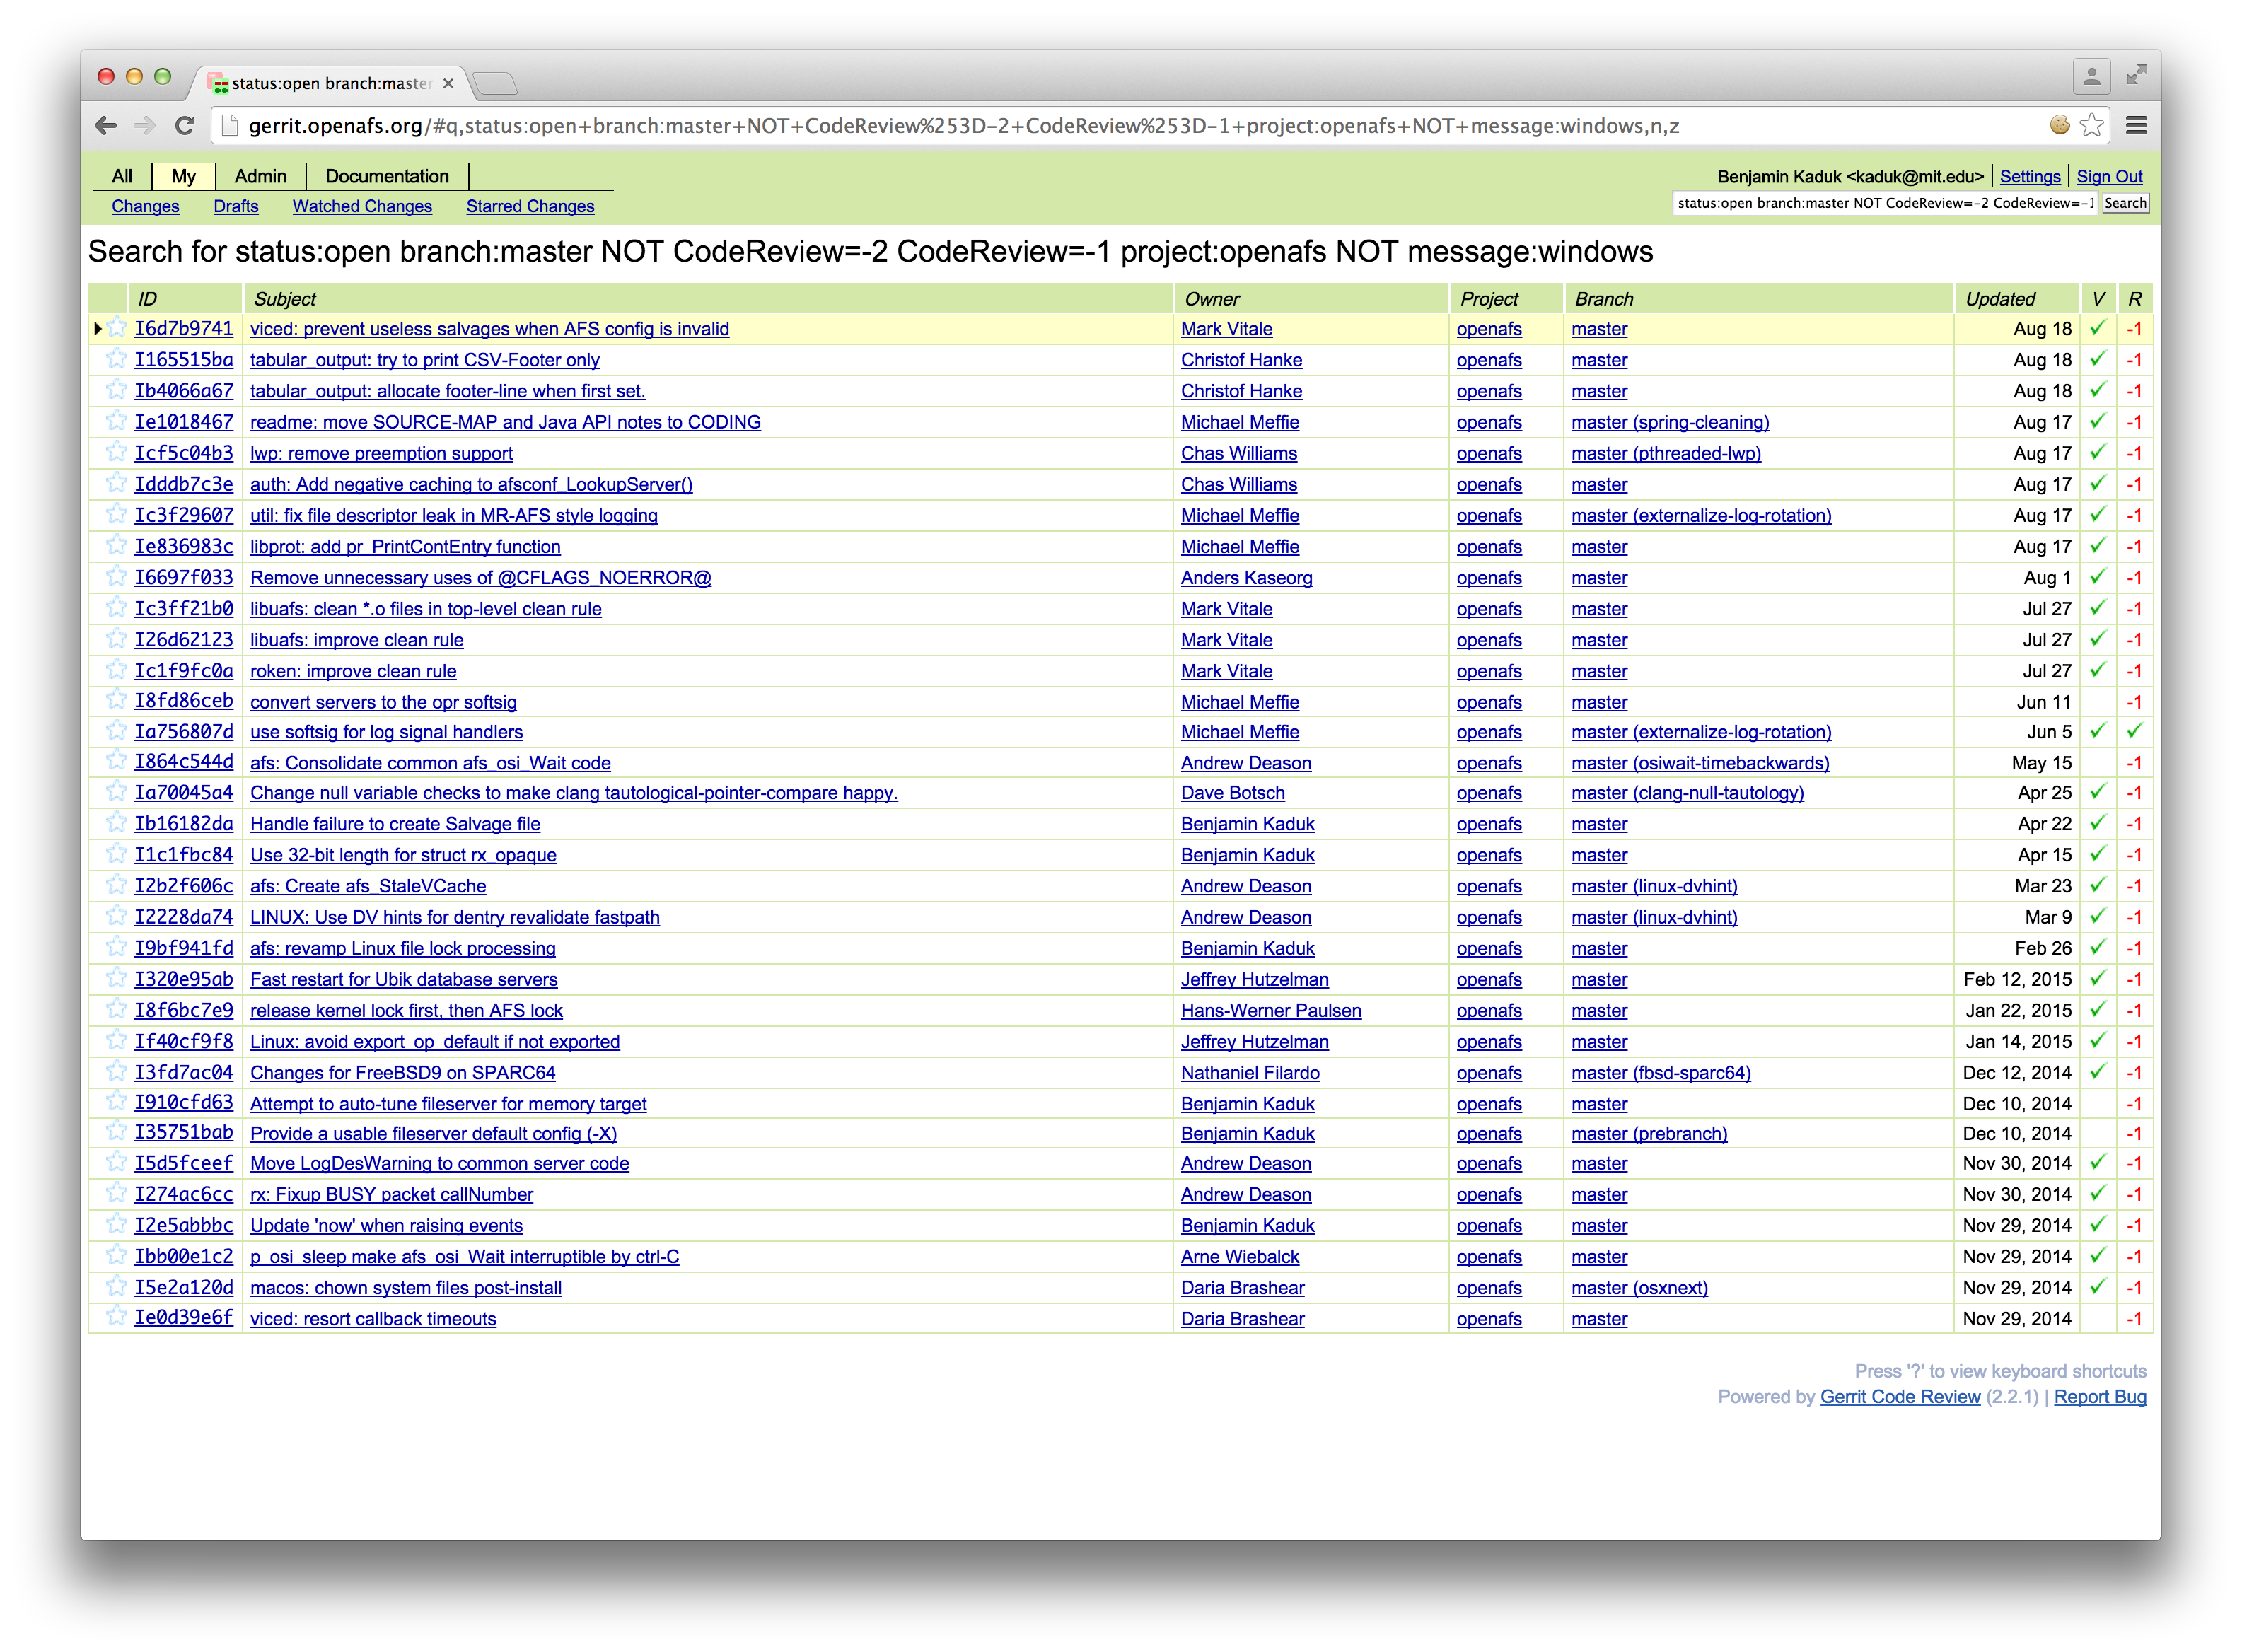
\includegraphics[width=4in]{gerrit-minusone}
\end{frame}

\begin{frame}
\frametitle{In gerrit needing rework}
33 changes with $-1$ review
\begin{itemize}
\item{viced: prevent useless salvages when AFS config is invalid}
\item{auth: Add negative caching to afsconf\_LookupServer()}
\item{convert servers to the opr softsig}
\item{Fast restart for Ubik database servers}
\pause
\item{Attempt to auto-tune fileserver for memory target}
\item{Provide a usable fileserver default config (-X)}
\pause
\item{p\_osi\_sleep make afs\_osi\_Wait interruptible by ctrl-C}
\end{itemize}
\end{frame}

\begin{frame}[fragile]
\frametitle{What's {\em not} in 1.8?}
\begin{itemize}
\item{kaserver (by default)}
\item{pam modules (by default)}
\item{Linux 2.4 support}
\item{Documentation for AIX-, HP-UX, and IRIX-specific installation in the
QuickStartGuide}
\item{NFS translator}
\item{A comprehensive test suite}
\item{\verb+afsd -settime+}
\item{\verb+libjuafs.a+ --- just use \verb+libuafs.a+}
\item{LWP fileserver}
\item{Cruft from MR-AFS in the bos utility}
\item{Netscape plugin (what is it???)}
\item{a \verb+-k+ argument to the fileserver}
\item{ZFS\_BOZONLOCK\_ENV}
\item{sunrpc compatibility in rxgen}
\end{itemize}
\end{frame}

\section{Getting to 2.0}

\subsection{rxgk}

\begin{frame}
\frametitle{Specification}
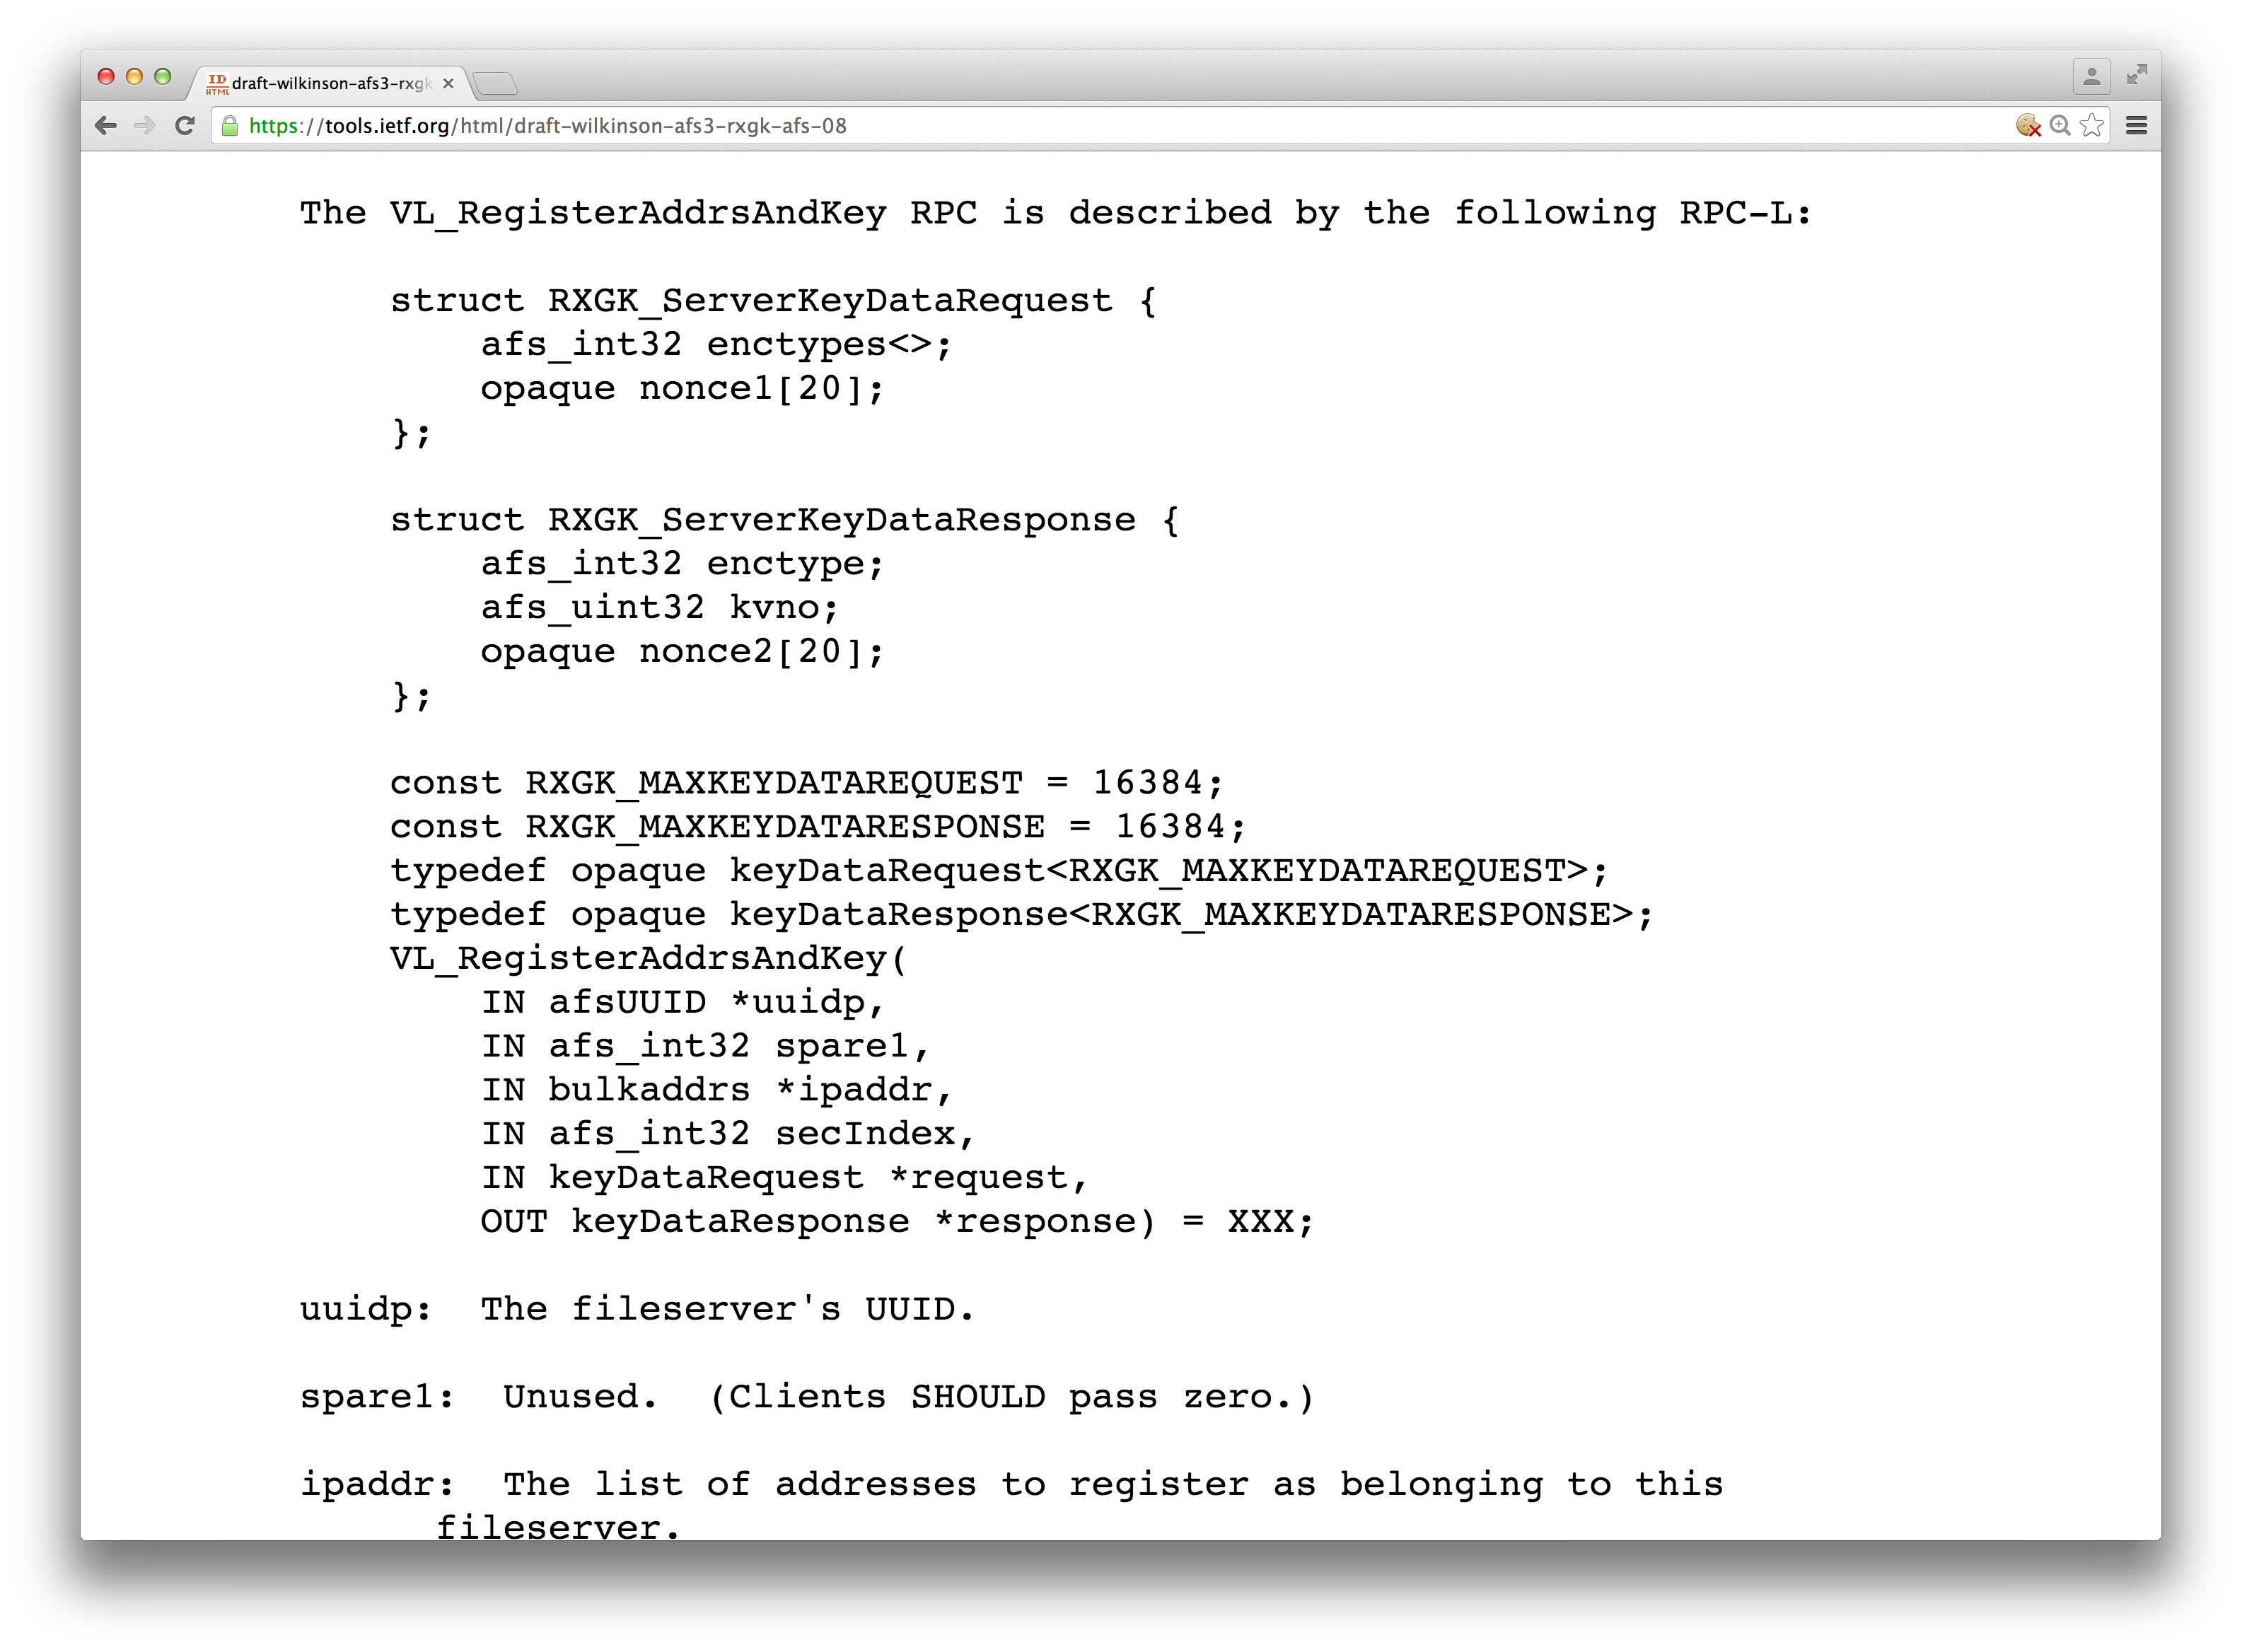
\includegraphics[width=4in]{rxgk-afs-snapshot}
\end{frame}

\begin{frame}
\frametitle{Implementation}
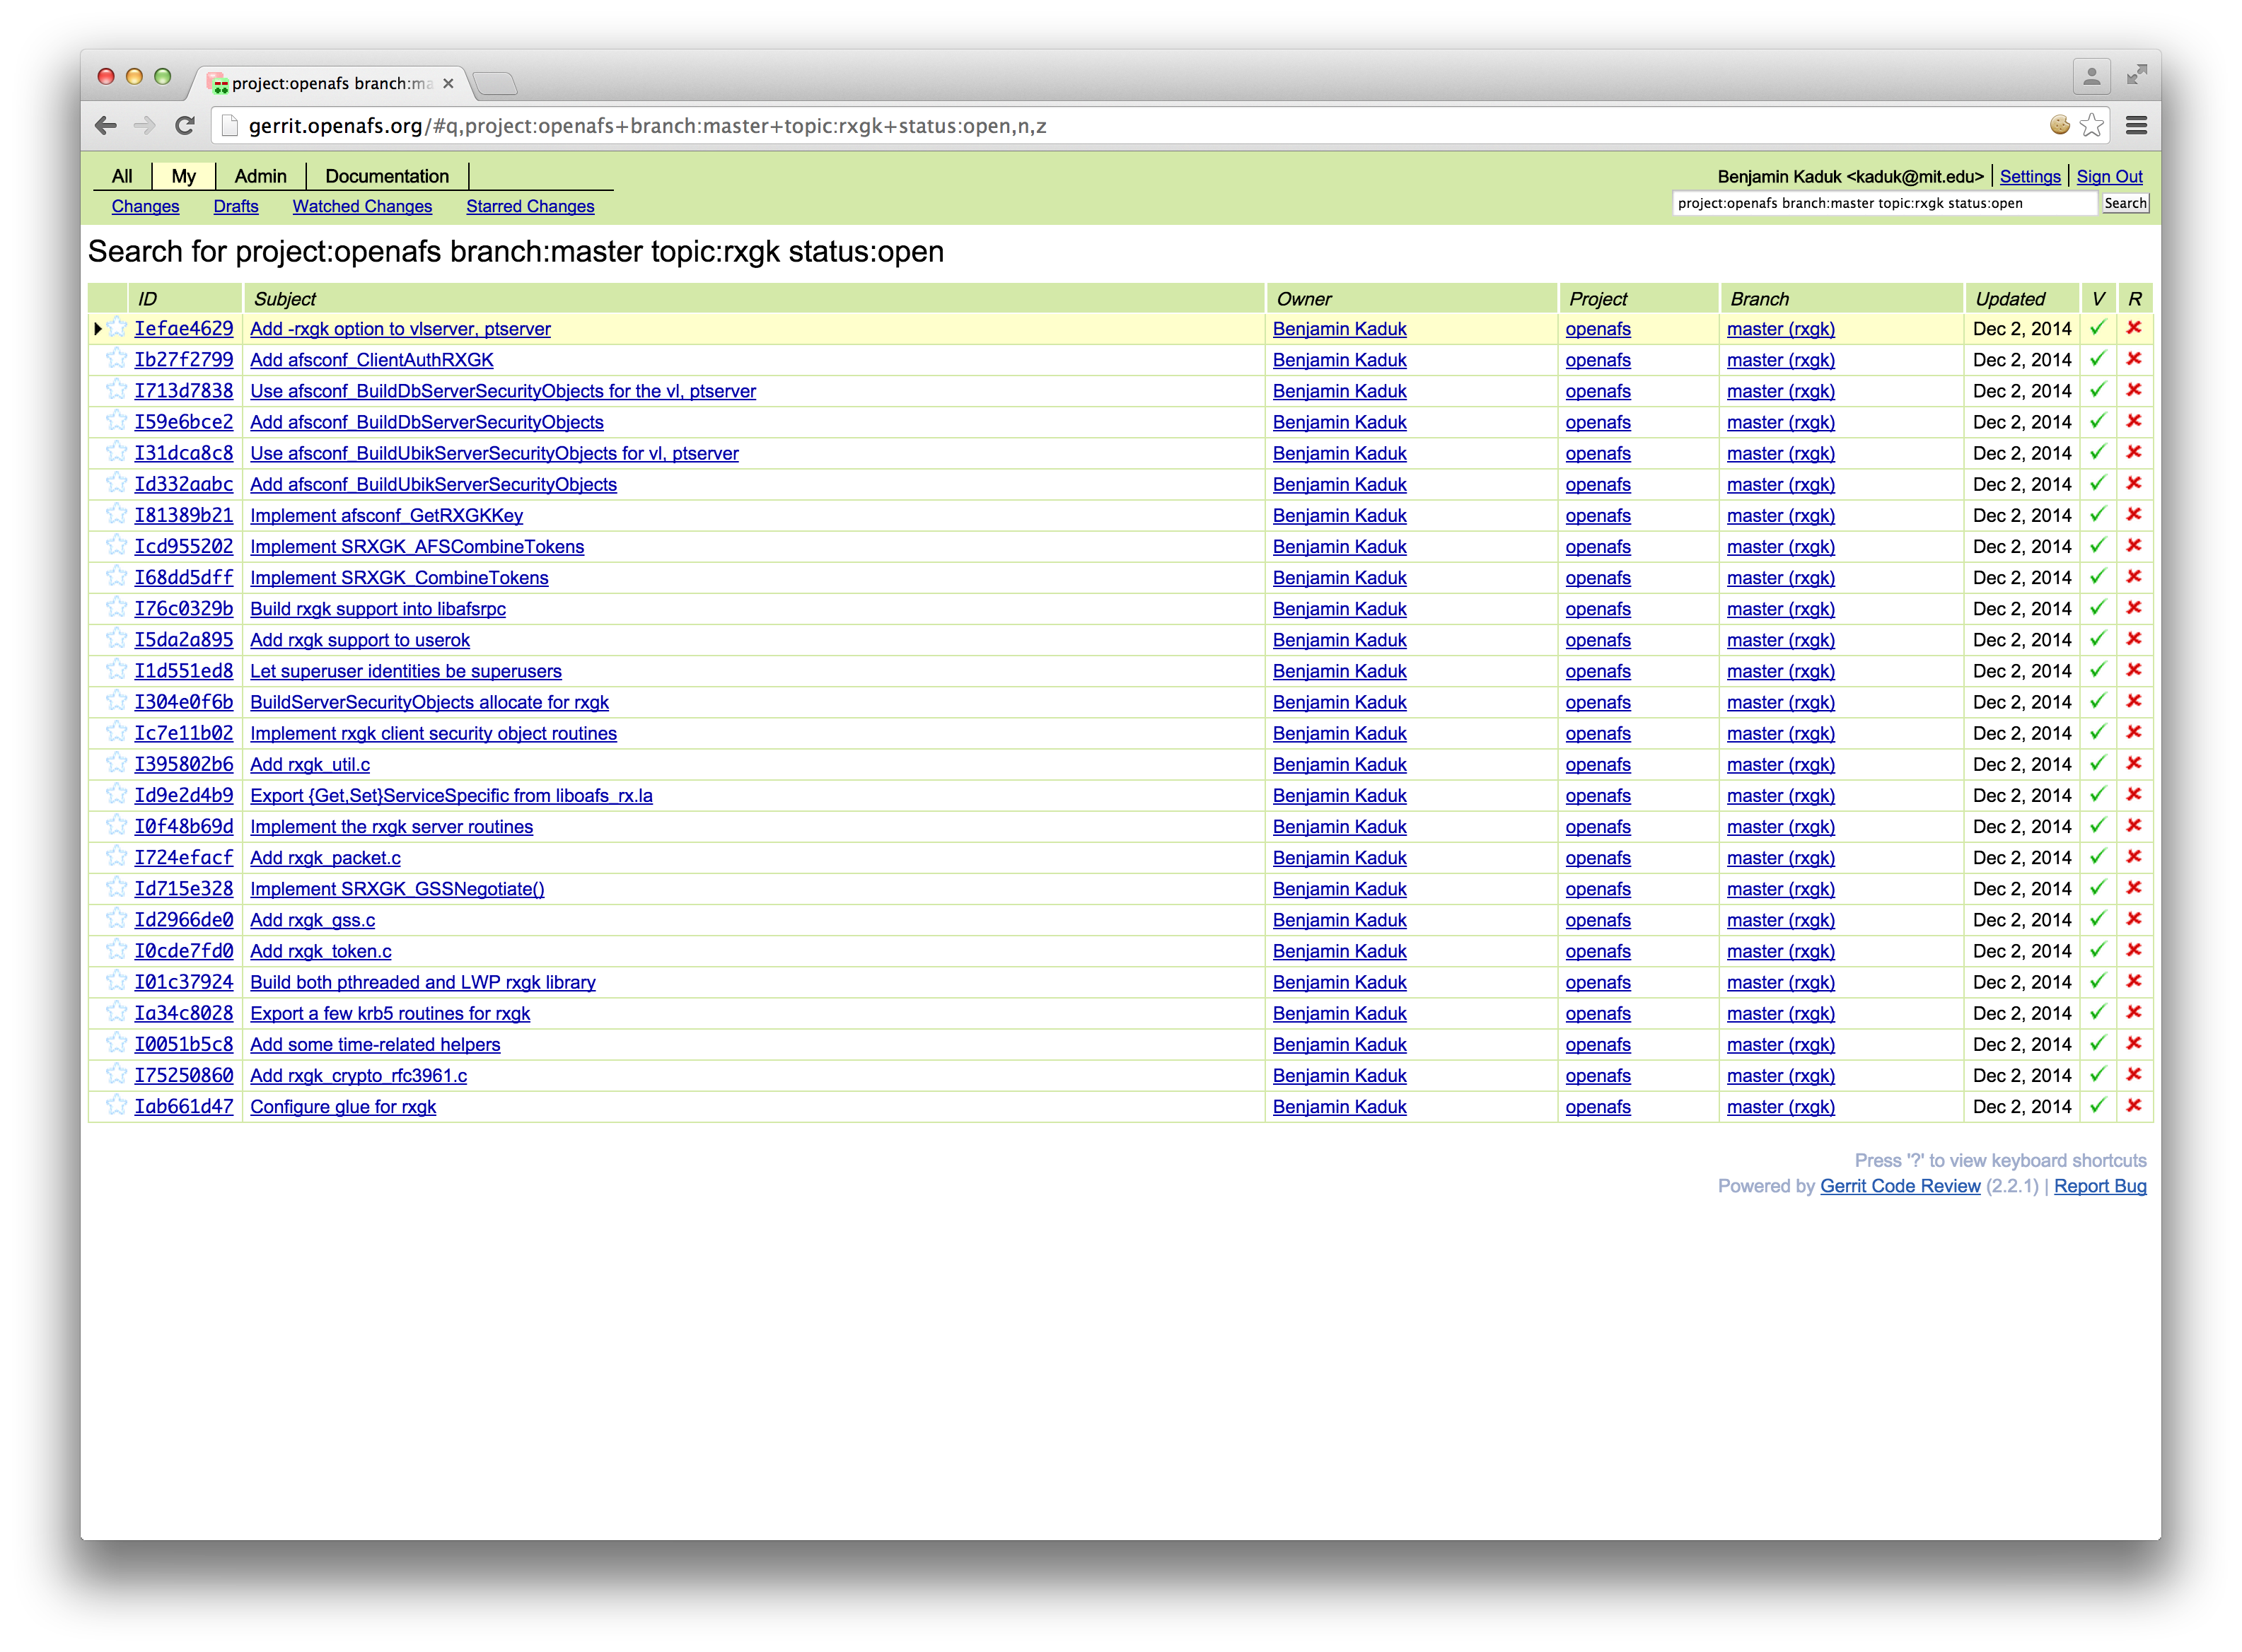
\includegraphics[width=4in]{gerrit-rxgk.png}
\end{frame}

\begin{frame}
\frametitle{Implementation}
\url{https://github.com/kaduk/openafs/commits/rxgkng}
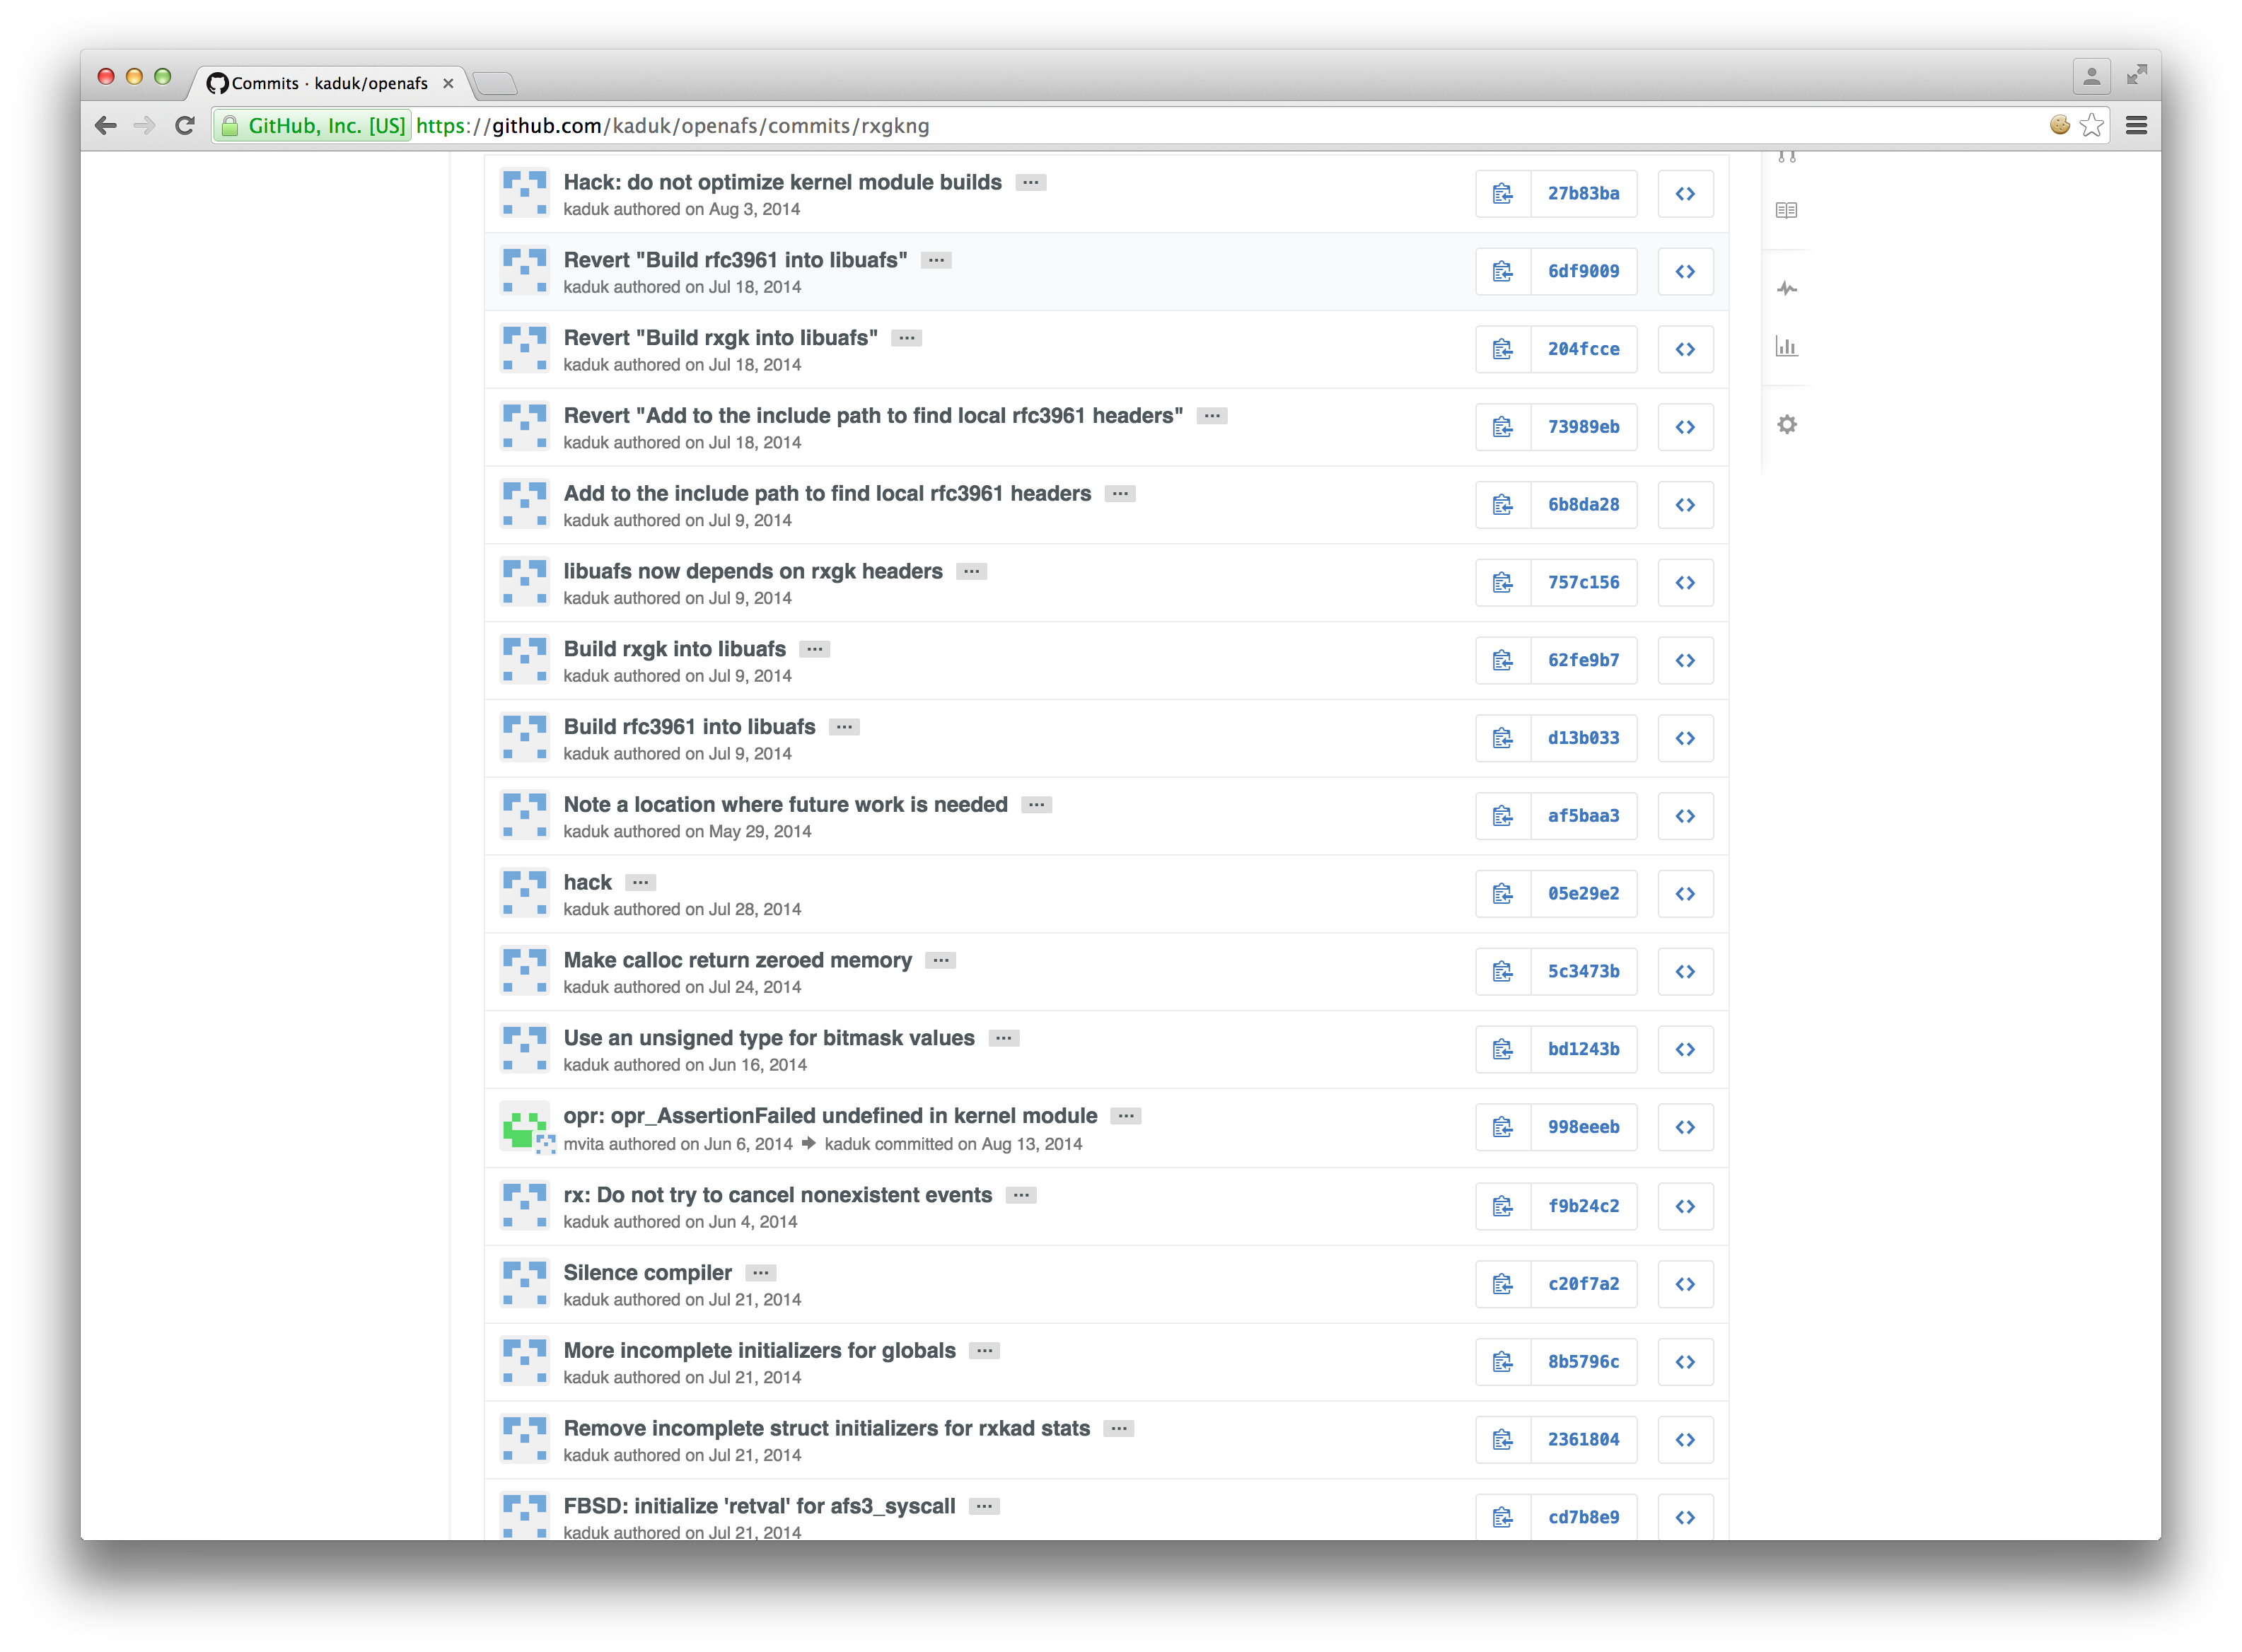
\includegraphics[width=4in]{github-rxgk}
\end{frame}

\subsection{IPv6}

\begin{frame}[fragile,shrink=-800]
\frametitle{Specification}
\verb+'()+
\end{frame}

\begin{frame}
\frametitle{Implementation}
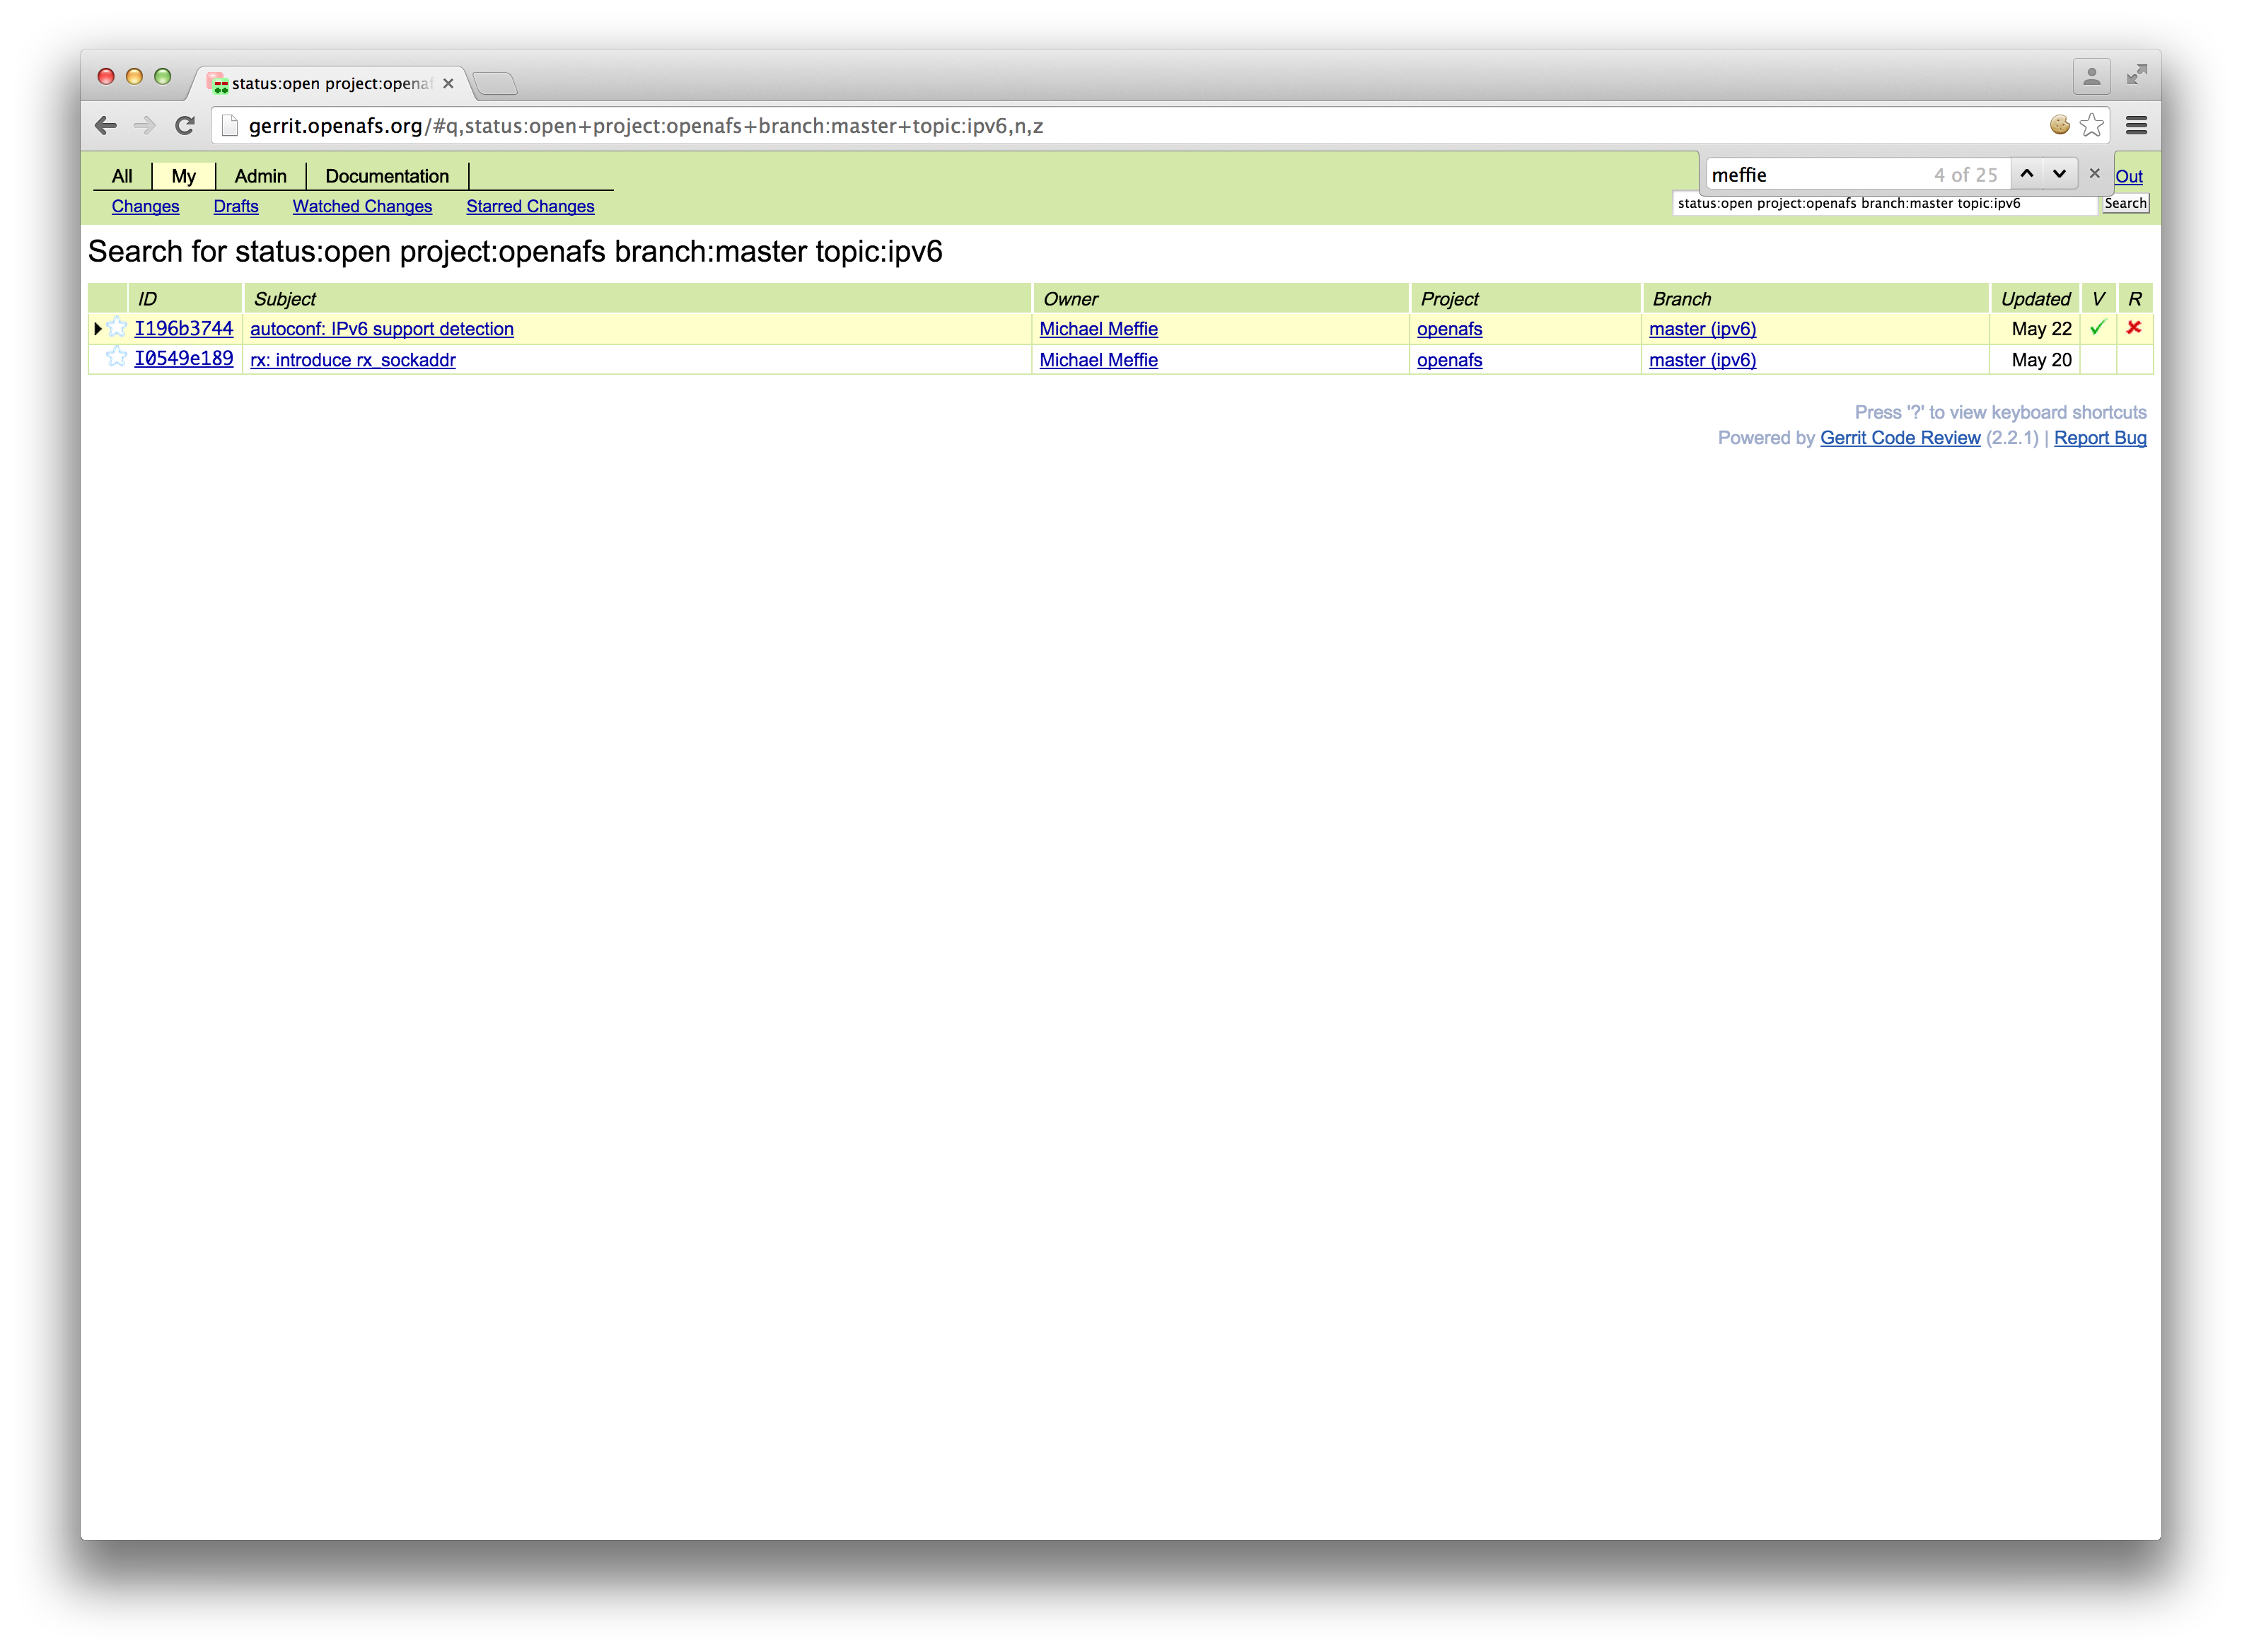
\includegraphics[width=4in]{gerrit-ipv6}
\end{frame}

\begin{frame}
\frametitle{Implementation}
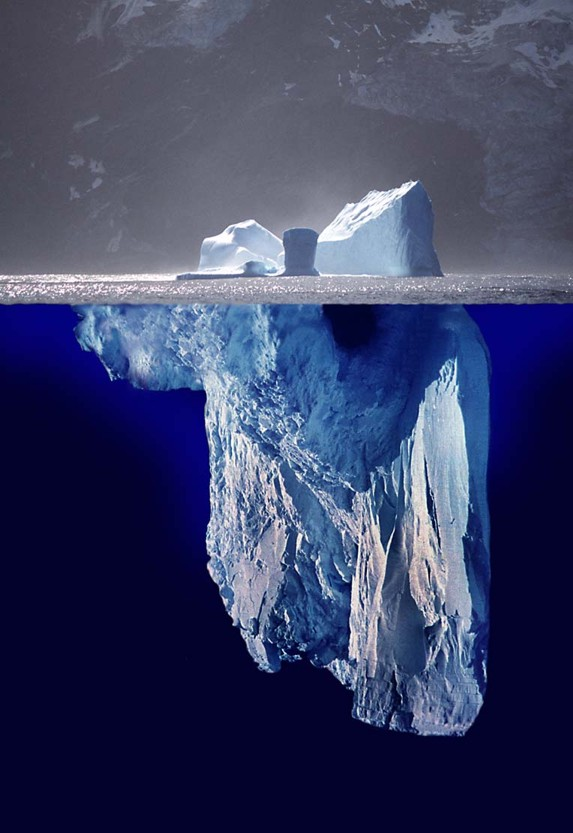
\includegraphics[height=3.3in]{iceberg}
\end{frame}

\subsection{\ldots}

\begin{frame}
\frametitle{Your Feature Here}
\begin{itemize}
\item{\sout{read-write replication}}
\item{\sout{per-file ACLs}}
\item{\ldots}
\end{itemize}
\end{frame}

\begin{frame}
\frametitle{}
\Large{Thanks!}
\end{frame}

\end{document}

% TODO
% make rxgen brief mode the only mode
